\section{Motivation}

Als Anwendungsszenario haben wir uns für ein Wetterdatensystem entschieden. Hierzu benutzen wir die Wetter-API von "OpenWeatherMap". Unser System gliedert sich in die 6 verschiedenen Komponenten WetterAPI, MOM, CEP, Datenbank, Android  User Client und ein User Client Webinterface. Mithilfe der WetterAPI werden die Wetterdaten für bestimmte Städte innerhalb Deutschlands über die MOM an die CEP geschickt. Die CEP verarbeitet und berechnet anhand der eingegangenen Wetterdaten bestimmte Benachrichtigungen (Alerts) für die User. Diese Alerts werden wiederum über die MOM an die User verteilt.  Zudem besteht die Möglichkeit sämtliche Wetterdaten und Alerts in einer Datenbank abzulegen. Ein Client User ist entweder per Android App oder Webinterface mit dem System bzw. der MOM verbunden.
Im folgenden Schaubild Abb.\ref{img:KomponentenKomplett} ist das Zusammenspiel der einzelnen Komponenten noch einmal grafisch visualisiert.

\begin{figure}[!ht]
	\centering
	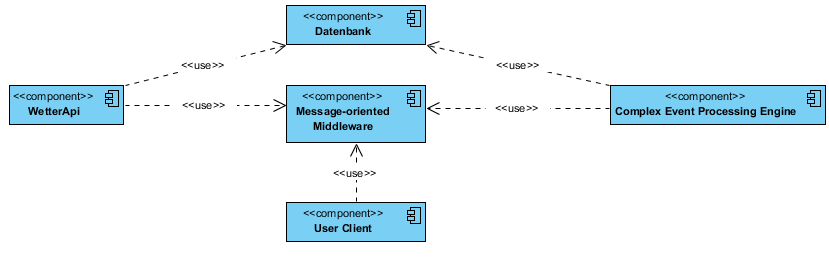
\includegraphics[width=1.0\textwidth]{Bilder/alleKomponenten.PNG}
	\caption{Wetter-API-Komponenten komplett}
	\label{img:KomponentenKomplett}
\end{figure}

Unser Wetter-API System stellt den User Clients neben einer Darstellung der tagesbezogenen Wetterdaten, eine Wettervorhersage der nächsten fünf Tage zur Verfügung. Im Unterschied zu herkömmlichen Wetterdiensten, bietet unser System zusätzlich noch Alerts an. Damit  können wir den User auf plötzliche Wetterumbrüche und beispielsweise vorzeitig Gefahrensituationen hinweisen und Empfehlungen aussprechen. 

Da der Traffic unseres Systems stark von den verbundenen Userzahlen und dem unkontrollierbaren Wetter abhängt, muss  das System auf verschiedene Lastsituationen angemessen reagieren können. Dies sind optimale Voraussetzungen für eine Lösung auf Basis eines Cloud Systems.

\subsection{Zielsetzung}
ToDo: Verweis auf 12 Faktor APP Standard !!! 
Die Tabelle soll am Anfang stehen, am besten in der Zielsetzung.
Die folgende Tabelle beschreibt die Kernanforderungen der 12 Faktor APP, 
\begin{table}[!ht]
  \centering
    \begin{minipage}{15cm}
      \centering
      \begin{tabular}{*{3}{|l|p{5.0cm}|p{5.0cm}}}\hline
      \multicolumn{3}{|c|}{\cellcolor[RGB]{200,200,200}12 Faktor APP Anforderungen} \\\hline
     \textbf{ID}&\textbf{Anforderung}&\textbf{Beschreibung}\\\hline
     1.&Codebase&Eine im Versionsmanagementsystem verwaltete Codebase, viele Deployments.\\
      \hline
     2.&Abhängigkeiten&Abhängigkeiten explizit deklarieren und isolieren.\\
     \hline
     3.&Konfiguration&Die Konfiguration in Umgebungsvariablen ablegen.\\
     \hline
     4.&Unterstützende Dienste&Unterstützende Dienste als angehängte Ressourcen behandeln.\\
     \hline 
     5.&Build, release, run&Build- und Run-Phase strikt trennen.\\
     \hline
     6.&Prozesse&Die App als einen oder mehrere Prozesse ausführen.\\
     \hline
      7.&Bindung an Ports&Dienste durch das Binden von Ports exportieren.\\
     \hline
      8.&Nebenläufigkeit&Mit dem Prozess-Modell skalieren.\\
     \hline
      9.&Einweggebrauch&Robuster mit schnellem Start und problemlosen Stopp.\\
     \hline
     10.&Dev-Prod-Vergleichbarkeit&Entwicklung, Staging und Produktion so ähnlich wie möglich halten.\\
     \hline     
     11.&Logs&Logs als Strom von Ereignissen behandeln.\\
     \hline
     12.&Admin-Prozesse&Admin/Management-Aufgaben als einmalige Vorgänge behandeln.\\
     \hline
      \end{tabular}
   \caption{12 Faktor App Anforderungen\cite{12:fac}}\label{tab:Anforderungen}
    \end{minipage}
\end{table}

\clearpage

\subsection{Die 12 Faktor-APP Anforderungen}